\documentclass[]{article}

% Imported Packages
%------------------------------------------------------------------------------
\usepackage{amssymb}
\usepackage{amstext}
\usepackage{amsthm}
\usepackage{amsmath}
\usepackage{enumerate}
\usepackage{fancyhdr}
\usepackage[margin=1in]{geometry}
\usepackage{graphicx}
\usepackage{extarrows}
\usepackage{setspace}
\usepackage{longtable}
%------------------------------------------------------------------------------
% Header and Footer
%------------------------------------------------------------------------------
\pagestyle{fancy}  
\lhead{T2 Group 10}
\chead{Software Requirements Specification}
\rhead{SFWRENG 3A04}
\renewcommand\headrulewidth{0.4pt}                                      
\renewcommand\footrulewidth{0.4pt}                                    
%------------------------------------------------------------------------------

% Title Details
%------------------------------------------------------------------------------
\title{\textbf{Boardzilla - Software Requirements Specification}}
\author{Matthew Paulin \\ paulinm \\ 400187147 \and
	Hargun Bedi \\ bedih \\ 400185463 \and
	Dylan Smith \\ smithd35 \\ 001314410 \and
	Chenwei Song \\ songc12 \\ 400124879 \and
	Tianzheng Mai \\ mait6 \\ 400143042
}
\date{\today}                               
%------------------------------------------------------------------------------

% Document
%------------------------------------------------------------------------------
\begin{document}
	\maketitle	 
	\newpage
	\tableofcontents
	\newpage
	
	\section{Introduction}
	\label{sec:introduction}
	% Begin Section
	
	This section of the SRS should provide an overview of the entire SRS.
	\\\\\\
	\textbf{
		\Large Boardzilla\\\\
		widgets }
	\begin{itemize}
		\item weather
		\item calendar
		\item sticky notes
		\item news (google news api)
		\item stock prices
	\end{itemize}
	\textbf{Functionality}
	\begin{itemize}
		\item Momentum-like welcome msg
		\item plus sign to add new widgets
		\item canvas starts blank, prompted with instructions to add first widget
		\item login to save data and widgets
	\end{itemize}
	\textbf{Implementation}
	\begin{itemize}
		\item React, JS, HTML5, CSS3
		\item bulma, materialize, or bootstrap for base styling
		\item hosting: AWS
		\item domain: ?
		\item backend: 
		\item db: MongoDB / other noSQL
		\item
	\end{itemize}
	\subsection{Purpose}
	\label{sub:purpose}
	% Begin SubSection
	This document will elucidate the requirements necessary to create Boardzilla. Some system requirements have been gathered from the project outline and others have been generated to create an acceptable final result. Additionally, this document will contain an explanation of the project and its constraints, the stakeholders of the project, as well as a quantitative measure of the desired finished product. The intended audience for this document include the team members who are developing the product, the Professor, Dr. Khedri, as well as any teaching assistants who will be grading this document.
	
	% \begin{enumerate}[a)]
	% 	\item Delineate the purpose of the SRS
	% 	\item Specify the intended audience for the SRS 
	% 	- team members, prof, TAs
	% \end{enumerate}
	% End SubSection
	
	\subsection{Scope}
	\label{sub:scope}
	% Begin SubSection
	The product being developed is called Boardzilla, an online application that will serve as a dashboard for a variety of pertinent information. Each user can have a unique dashboard containing their desired widgets from the available options. These options include: a weather widget, a sticky notes widget, a calendar widget, a news widget, and an widget showing live stock prices. This application will serve as a daily briefing to users, presenting live, relevant, and customizable information that is all aggregated on a single page. 
	% \begin{enumerate}[a)]
	% 	\item Identify the software product(s) to be produced by name (e.g., Host DBMS, Report Generator, etc.)
	% 	\item Explain what the software product(s) will, and, if necessary, will not do
	% 	\item Describe the application of the software being specified, including relevant benefits, objectives, and goals
	% 	\item Be consistent with similar statements in higher-level specifications (e.g., the system requirements specification), if they exist
	% \end{enumerate}
	
	% End SubSection
	
	\subsection{Definitions, Acronyms, and Abbreviations}
	\label{sub:definitions_acronyms_and_abbreviations}
	% Begin SubSection
	\begin{itemize}
		% 	\item Provide the definitions of all terms, acronyms, and abbreviations required to properly interpret the SRS
		\item \textbf{Dashboard}: A user interface or web page that gives a current summary, usually in graphic, easy-to-read form, of key information relating to progress and performance, especially of a business or website. %\url{https://www.dictionary.com/browse/dashboard}
		
		\item \textbf{Widget}: An element of a user interface that displays information or provides a specific way for a user to interact with an application. %\url{https://whatis.techtarget.com/definition/widget}
	\end{itemize}
	% End SubSection
	
	\subsection{References}
	\label{sub:references}
	% Begin SubSection
	% \begin{enumerate}[a)]
	% 	\item Provide a complete list of all documents referenced elsewhere in the SRS
	% 	\item Identify each document by title, report number (if applicable), date, and publishing organization
	% 	\item Specify the sources from which the references can be obtained
	% \end{enumerate}
	% End SubSection
	
	\subsection{Overview}
	\label{sub:overview}
	% Begin SubSection
	The remainder of this document will provide an overall description of our product, a use case diagram depicting the business events, the functional and non-functional requirements, and the division of labour. 
	%\begin{enumerate}[a)]
		% 	\item Describe what the rest of the SRS contains
		% 	\item Explain how the SRS is organized
		
	%	\end{enumerate}
	% End SubSection
	
	% End Section
	
	\section{Overall Description}
	\label{sec:overall_description}
	% Begin Section
	
	% This section of the SRS should describe the general factors that affect the product and its requirements. It does not state specific requirements; it provides a background for those requirements and makes them easier to understand.
	
	\subsection{Product Perspective}
	\label{sub:product_perspective}
	% Begin SubSection
	Our system will provide users with a large variety of widgets to customize their dashboard. Similar dashboard applications are focused on relaying analytical information such as team or product statistics. Boardzilla's widgets provide users with options relevant to broader demographics rather than individual businesses. These widgets can then be combined and configured by the user, providing them with a dashboard that is unique to them. The standalone versions of the widgets such as Google News or The Weather Network provide the same information but are lacking in convenience due to being largely isolated applications. The system will interface with external databases that contain news data, weather data, stock data, and calendar data. %\url{https://medium.com/theymakedesign/best-web-design-inspiration-dashboards-d87015ffb711} In addition, our dashboard's ability to be customized does not sacrifice any functionality or usability to the overall application.
	%\begin{enumerate}[a)]
		% 	\item Put the product into perspective with other related products, i.e., context
		% 	\item If the product is independent and totally self-contained, it should be stated here
		% 	\item If the SRS defines a product that is a component of a larger system, as frequently occurs, then this subsection should relate the requirements of that larger system to functionality of the software and should identify interfaces between that system and the software
		% 	\item A block diagram showing the major components of the larger system, interconnections, and external interfaces can be helpful
		
	%\end{enumerate}
	
	% End SubSection
	
	\subsection{Product Functions}
	\label{sub:product_functions}
	% Begin SubSection
	When a user navigates to Boardzilla, they will be presented with a login page. If they are unregistered, they will have to first register before being able to access their personalized dashboard. Once logged in, a user will be able to see a welcome page greeting the user personally with a friendly message. The app will also display the user's widgets in their chosen configuration. By dragging the widgets around the screen, the positioning and layering can be adjusted to suit the user's needs. Each widget will have an ability for minimization or deletion and there will also be a menu to add additional widgets. The available widgets will include weather, stock, calendar, news and sticky notes. When adding new widgets, the user must select specific widget options if necessary. All of the user's dashboard and individual widget customization will be saved in the cloud and accessible through their account on multiple machines.
	% \begin{enumerate}[a)]
	% \begin{itemize}
	%     \item Boardzilla will provide a welcome page greeting the user when opening the app.
	%     \item Boardzilla will display the user's chosen widgets in their chosen layout and layering.
	%     \item Boardzilla will provide a menu enabling users to add to additional widgets or remove existing ones from their personal dashboard.
	%     \item Boardzilla will allow users to adjust the positioning and layering of the widgets on their personal dashboard.
	%     \item The list of available widgets will include weather, stock, calendar, news and sticky notes.
	%     \item Widgets will be able to be minimized and displayed in a task bar.
	%     \item Boardzilla will store widget selection and positioning for each user in the cloud. 
	%     \item Users will create an account which will save their dashboard.
	%     \item Users will be able to log in to their account to display their dashboard on different machines.
	% \end{itemize}
	
	% 	\item Provide a summary of the major functions that the software will perform. 
	% 	\begin{itemize}
	% 		\item \textbf{Example}: A SRS for an accounting program may use this part to address customer account maintenance, customer statement, and invoice preparation without mentioning the vast amount of detail that each of those functions requires.
	% 	\end{itemize}
	% 	\item Functions should be organized in a way that makes the list of functions understandable to the customer or to anyone else reading the document for the first time
	% 	\item Textual or graphical methods can be used to show the different functions and their relationships
	% 	\begin{itemize}
	% 		\item Such a diagram is not intended to show a design of a product, but simply shows the logical relationships among variables
	% 	\end{itemize} 
	% \end{enumerate}
	% End SubSection
	
	\subsection{User Characteristics}
	\label{sub:user_characteristics}
	% Begin SubSection
	Boardzilla will be designed to appeal to everyone in the English speaking world, the only requisite knowledge being how to use a computer and web browser. To that end, intended users of Boardzilla will not be required to have any other technical background or education besides an intermediate understanding of the English language. Additionally, prior experience with our application will not be required because all relevant information will be provided to the user upon registration. 
	% The users will choose widgets by clicking and dragging icons according to their own need and point of interest in a way that Boardzilla could serve them the best.
	% \begin{enumerate}[a)]
	% 	\item Describe those general characteristics of the intended users of the product including educational level, experience, and technical expertise
	% 	\item Do not state specific requirements, but rather provide the reasons why certain specific requirements are later specified
	% \end{enumerate}
	% End SubSection
	
	\subsection{Constraints}
	\label{sub:constraints}
	% Begin SubSection
	\begin{itemize}
		% \item The user must have internet access to log in to their account and gain access to their saved widget selection and layout.
		\item Boardzilla must be given internet access to fetch data from external databases in order to populate the widgets with data.
		\item Boardzilla must obey local laws and regulations.
		\item Boardzilla must follow the terms of service of all external APIs.
	\end{itemize}
	% \begin{enumerate}[a)]
	% 	\item Provide a general description of any other items that will limit the developer's options
	% \end{enumerate}
	% End SubSection
	
	\subsection{Assumptions and Dependencies}
	\label{sub:assumptions_and_dependencies}
	% Begin SubSection
	Assumptions:
	\begin{itemize}
		\item Users will know English or have a browser capable of translating to their spoken language.
		% \item Boardzilla will work on a browser.
	\end{itemize}
	Dependencies:
	\begin{itemize}
		\item Google API -- expand
		% \item Weather, news, stock, and calendar data will be fetched from external APIs.
		% \item Widget data will be dependant on the availability of data from the APIs.
		% \item The software will be dependent on existing languages, frameworks, and technologies.
	\end{itemize}
	\begin{enumerate}[a)]
		\item List each of the factors that affect the requirements stated in the SRS
		\item These factors are not design constraints on the software but are, rather, any changes to them that can affect the requirements in the SRS
		\begin{itemize}
			\item \textbf{Example}: An assumption may be that a specific operating system will be available on the hardware designated for the software product. If, in fact, the operating system is not available, the SRS would then have to change accordingly.
		\end{itemize}
	\end{enumerate}
	% End SubSection
	
	\subsection{Apportioning of Requirements}
	\label{sub:apportioning_of_requirements}
	% Begin SubSection
	In future versions we will:  
	\begin{itemize}
		\item Enable the user to choose from a wider variety of widgets.
		\item Add multiple language and region support for the text within the application.
		\item Increase the level of accessibility for physically or mentally impaired users.
		% \item Add additional browser support (i.e. Internet Explorer 8, Opera, Tor).
		\item Allow users to see previously retrieved information in an offline version of the application.
		\item Allow users to save and access multiple layout configurations.
	\end{itemize}
	% \begin{enumerate}[a)]
	% 	\item Identify requirements that may be delayed until future versions of the system
	% \end{enumerate}
	% End SubSection
	
	% End Section
	\newpage
	\section{Use Case Diagram}
	\label{sec:use_case_diagram}
	% Begin Section
	This section should provide a use case diagram for your application. 
	\begin{enumerate}[a)]
		\item Each use case appearing in the diagram should be accompanied by a text description. 
		
		\begin{figure}[h!]
			\begin{center}
				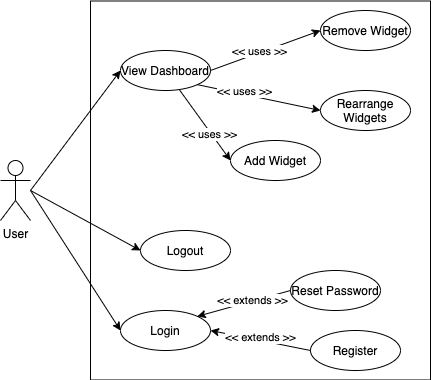
\includegraphics[width=0.6\textwidth]{Usecase.png}
			\end{center}
			\caption{Use Case Diagram}
			\label{fig:use case diagram}
		\end{figure}
	\end{enumerate}
	% End Section
	
	\section{Functional Requirements}
	\label{sec:functional_requirements}
	% Begin Section
	% This section of the SRS should contain all of the software requirements to a level of detail sufficient to enable designers to design a system to satisfy those requirements, and testers to test that the system satisfies those requirements. Throughout this section, every stated requirement should be externally perceivable by users, operators, or other external systems. These requirements should include at a minimum a description of every input (stimulus) into the system, every output (response) from the system, and all functions performed by the system in response to an input or in support of an output.
	
	% You normally have two options for organizing your functional requirements:
	% \begin{enumerate}
	% 	\item Organize first by \emph{business events}, then by \emph{viewpoints}
	% 	\item Organize first by \emph{viewpoints}, then by \emph{business events}
	% \end{enumerate}
	% Choose the one which makes the most sense.
	
	% business events: user wants to register, user wants to add a widget, user wants to delete a widget, user logs in for the first time, user logs out
	
	% For example, if you wish to organization by business events:
	
	
	% \underline{OR}, if you wish to organization by viewpoints:
	\begin{enumerate}[{VP}1]
		\item User
		\begin{enumerate}[{BE}1]
			\item User wants to view their dashboard
			\begin{enumerate}
				\item The system will check if the user is logged in to their account with the system.
				\item If the user is not logged in, the system will redirect the user to the system registration page.
				\item The system will fetch the user's widgets from the internal database.
				\item The system will display the user's  widgets in accordance with the user's chosen positioning.
				\item The system will display the add and remove widget options.
				\item The system will update the widgets with current information.
				\item The users will be able to access more information by hovering over the associated help icons.
			\end{enumerate}
			\item User registers for an account
			\begin{enumerate}
				\item The system will provide the user with a sign up form.
				\item The system will verify the validity of the information and will create an account in the database if the information is valid.   
				\item The system will display an error message upon an invalid registration.
				\item The system will redirect the user to a newly created, empty dashboard and will display system instructions.
			\end{enumerate}
			\item User attempts to login to the system
			\begin{enumerate}
				\item The system will display a login form.
				\item The system will verify that correct login information was provided.
				\item The system will redirect the user to their own dashboard. 
				\item The system will display an error message after an invalid login attempt.
			\end{enumerate}
			\item User wants to add a widget to their dashboard
			\begin{enumerate}
				\item The system will provide the user with a list of possible widgets. 
				\item The system will allow the user to input a widget selection and will redirect them to the setup page for that widget.
				\item After widget configuration, the system will prompt the user to place the widget on their dashboard.
				\item The system will display an error message indicating any incorrect widget parameters.
				\item The system will fetch the widget data.
				\item The widget and its parameters will be added to the system's database.
			\end{enumerate}
			\item User wants to remove a widget from their dashboard
			\begin{enumerate}
				\item The system will provide the user with a list of existing widgets to delete. 
				\item The system will remove the selected widget from the database.
				\item The system will remove the selected widget from the dashboard
			\end{enumerate}
			\item User wants to log out of the application
			\begin{enumerate}
				\item The system will invalidate the user's session.
				\item The user will be redirected to the login page.
			\end{enumerate}
			\item User wants to reset their password
			\begin{enumerate}
				\item The system will send a password reset email containing a temporary password.
				\item The user will be redirected to the change password page where they can modify their password.
			\end{enumerate}
			\item User wants to modify their dashboard layout
			\begin{enumerate}
				\item The positioning of the widgets will be updated in the system's database.
				\item The display will reflect the updated widget positioning.
			\end{enumerate}
		\end{enumerate}
	\end{enumerate}
	
	% % End Section
	
	\section{Non-Functional Requirements}
	\label{sec:non-functional_requirements}
	% Begin Section
	\subsection{Look and Feel Requirements}
	\label{sub:look_and_feel_requirements}
	% Begin SubSection
	
	\subsubsection{Appearance Requirements}
	\label{ssub:appearance_requirements}
	% Begin SubSubSection
	\begin{enumerate}[{LF}1. ]
		\item The system shall use modern styling whenever possible.
		\item The system shall be visually appealing to 77\% of users.
	\end{enumerate}
	% End SubSubSection
	
	\subsubsection{Style Requirements}
	\label{ssub:style_requirements}
	% Begin SubSubSection
	\begin{enumerate}[{LF}1. ]
		\item The text size and font must be legible at a normal computer viewing distance.
		\item The fonts, colours, and icons must remain consistent throughout the system.
	\end{enumerate}
	% End SubSubSection
	
	% End SubSection
	
	\subsection{Usability and Humanity Requirements}
	\label{sub:usability_and_humanity_requirements}
	% Begin SubSection
	
	\subsubsection{Ease of Use Requirements}
	\label{ssub:ease_of_use_requirements}
	% Begin SubSubSection
	\begin{enumerate}[{UH}1. ]
		\item Any buttons must be large enough to be located and pressed within 5 seconds.
		\item The users must be presented with general instructions when logging in for the first time.
		\item The language should be understandable to anyone with a fifth grade level of reading comprehension.
	\end{enumerate}
	% End SubSubSection
	
	\subsubsection{Personalization and Internationalization Requirements}
	\label{ssub:personalization_and_internationalization_requirements}
	% Begin SubSubSection
	\begin{enumerate}[{UH}1. ]
		\item Boardzilla must allow users to adjust the positioning and layering of the widgets on their personal dashboard.
		\item Widgets must accept valid parameters from users.
	\end{enumerate}
	% End SubSubSection
	
	\subsubsection{Learning Requirements}
	\label{ssub:learning_requirements}
	% Begin SubSubSection
	\begin{enumerate}[{UH}1. ]
		\item The user interface must be understood by a user within 10 minutes of system use.
	\end{enumerate}
	% End SubSubSection
	
	\subsubsection{Understandability and Politeness Requirements}
	\label{ssub:understandability_and_politeness_requirements}
	% Begin SubSubSection
	\begin{enumerate}[{UH}1. ]
		\item The symbols must convey the correct meaning to users 95\% of the time.
		\item The language in the app must be grammatically correct 99\% of the time.
	\end{enumerate}
	% End SubSubSection
	
	\subsubsection{Accessibility Requirements}
	\label{ssub:accessibility_requirements}
	% Begin SubSubSection
	\begin{enumerate}[{UH}1.]
		\item Any adjacent colours used within the user interface must appear distinct to users afflicted with colour blindness.
	\end{enumerate}
	% End SubSubSection
	
	% End SubSection
	\subsection{Performance Requirements}
	\label{sub:performance_requirements}
	% Begin SubSection
	
	\subsubsection{Speed and Latency Requirements}
	\label{ssub:speed_and_latency_requirements}
	% Begin SubSubSection
	\begin{enumerate}[{PR}1. ]
		\item The system shall respond to network requests with the necessary information in less than 3 seconds 99\% of the time.
		\item A request to fetch user data from the external \textbf{APIs} must be sent in under 10 seconds 99\% of the time.
		\item 
	\end{enumerate}
	% End SubSubSection
	
	\subsubsection{Safety-Critical Requirements}
	\label{ssub:safety_critical_requirements}
	% Begin SubSubSection
	\begin{enumerate}[{PR}1. ]
		\item N/A
	\end{enumerate}
	% End SubSubSection
	
	\subsubsection{Precision or Accuracy Requirements}
	\label{ssub:precision_or_accuracy_requirements}
	% Begin SubSubSection
	\begin{enumerate}[{PR}1. ]
		\item The system must show correct widget information 99\% of the time.
		\item The database must store current information 99.9\% of the time.
	\end{enumerate}
	% End SubSubSection
	
	\subsubsection{Reliability and Availability Requirements}
	\label{ssub:reliability_and_availability_requirements}
	% Begin SubSubSection
	\begin{enumerate}[{PR}1. ]
		\item Boardzilla shall be available for use 99.99\% of the time.
		\item The system shall require internet access to function.
	\end{enumerate}
	% End SubSubSection
	
	\subsubsection{Robustness or Fault-Tolerance Requirements}
	\label{ssub:robustness_or_fault_tolerance_requirements}
	% Begin SubSubSection
	\begin{enumerate}[{PR}1.]
		\item Boardzilla must display data consistently across supported devices.
		\item The system shall remain visible, but with stale data in the case of internet loss.
		\item The system shall notify active users in the case of a system failure, or loss of connectivity to the system.
	\end{enumerate}
	% End SubSubSection
	
	\subsubsection{Capacity Requirements}
	\label{ssub:capacity_requirements}
	% Begin SubSubSection
	\begin{enumerate}[{PR}1. ]
		\item The system shall be able to handle up to 100 users concurrently.
	\end{enumerate}
	% End SubSubSection
	
	\subsubsection{Scalability or Extensibility Requirements}
	\label{ssub:scalability_or_extensibility_requirements}
	% Begin SubSubSection
	\begin{enumerate}[{PR}1. ]
		\item The system shall be designed such that additional widgets can be added in future versions without modifying more than 10\% of existing software.
	\end{enumerate}
	% End SubSubSection
	
	\subsubsection{Longevity Requirements}
	\label{ssub:longevity_requirements}
	% Begin SubSubSection
	\begin{enumerate}[{PR}1. ]
		\item The system shall remain online for at least 2 years after software delivery. 
	\end{enumerate}
	% End SubSubSection
	
	% End SubSection
	
	\subsection{Operational and Environmental Requirements}
	\label{sub:operational_and_environmental_requirements}
	% Begin SubSection
	
	\subsubsection{Expected Physical Environment}
	\label{ssub:expected_physical_environment}
	% Begin SubSubSection
	\begin{enumerate}[{OE}1. ]
		\item Boardzilla shall be operable in any physical environment that mobile phones or desktop computers can be operated in.
	\end{enumerate}
	% End SubSubSection
	
	\subsubsection{Requirements for Interfacing with Adjacent Systems}
	\label{ssub:requirements_for_interfacing_with_adjacent_systems}
	% Begin SubSubSection
	\begin{enumerate}[{OE}1. ]
		\item The application shall interface with APIs that provide widget data at no cost.
	\end{enumerate}
	% End SubSubSection
	
	\subsubsection{Productization Requirements}
	\label{ssub:productization_requirements}
	% Begin SubSubSection
	\begin{enumerate}[{OE}1. ]
		\item N/A
	\end{enumerate}
	% End SubSubSection
	
	\subsubsection{Release Requirements}
	\label{ssub:release_requirements}
	% Begin SubSubSection
	\begin{enumerate}[{OE}1. ]
		\item The system must have 90\% of software issues patched before release.
	\end{enumerate}
	% End SubSubSection
	
	% End SubSection
	
	\subsection{Maintainability and Support Requirements}
	\label{sub:maintainability_and_support_requirements}
	% Begin SubSection
	
	\subsubsection{Maintenance Requirements}
	\label{ssub:maintenance_requirements}
	% Begin SubSubSection
	\begin{enumerate}[{MS}1. ]
		\item System updates shall not keep the system down for longer than 10 minutes.
		\item The system shall have an uptime of 99.99\%.
	\end{enumerate}
	% End SubSubSection
	
	\subsubsection{Supportability Requirements}
	\label{ssub:supportability_requirements}
	% Begin SubSubSection
	\begin{enumerate}[{MS}1. ]
		\item The system's instructions shall explain 99\% of scenarios.
	\end{enumerate}
	% End SubSubSection
	
	\subsubsection{Adaptability Requirements}
	\label{ssub:adaptability_requirements}
	% Begin SubSubSection
	\begin{enumerate}[{MS}1. ]
		\item N/A
	\end{enumerate}
	% End SubSubSection
	% End SubSection
	
	\subsection{Security Requirements}
	\label{sub:security_requirements}
	% Begin SubSection
	
	\subsubsection{Access Requirements}
	\label{ssub:access_requirements}
	% Begin SubSubSection
	\begin{enumerate}[{SR}1. ]
		\item The system shall only allow access if a valid username and password are entered.
		\item The system shall only provide a user with access to their dashboard.
	\end{enumerate}
	% End SubSubSection
	
	\subsubsection{Integrity Requirements}
	\label{ssub:integrity_requirements}
	% Begin SubSubSection
	\begin{enumerate}[{SR}1. ]
		% 	\item The system will not allow users to modify API's.
		\item The system must sanitize all data that is collected from users.
		\item The system must employ rate limiting to cap the addition of widgets to one widget per twenty seconds per user.
		\item The user must not be able to manipulate other user's data.
	\end{enumerate}
	% End SubSubSection
	
	\subsubsection{Privacy Requirements}
	\label{ssub:privacy_requirements}
	% Begin SubSubSection
	\begin{enumerate}[{SR}1. ]
		\item The system must not release user information to any third party.
		\item The system shall not store unencrypted user passwords.
		\item The system shall not collect any unnecessary user data.
	\end{enumerate}
	% End SubSubSection
	
	\subsubsection{Audit Requirements}
	\label{ssub:audit_requirements}
	% Begin SubSubSection
	\begin{enumerate}[{SR}1. ]
		\item After a security audit, at least 90\% of the changes should be made within a month.
	\end{enumerate}
	% End SubSubSection
	
	\subsubsection{Immunity Requirements}
	\label{ssub:immunity_requirements}
	% Begin SubSubSection
	\begin{enumerate}[{SR}1. ]
		\item Software security patches must be installed within a week of their release.
	\end{enumerate}
	% End SubSubSection
	
	% End SubSection
	
	\subsection{Cultural and Political Requirements}
	\label{sub:cultural_and_political_requirements}
	% Begin SubSection
	
	\subsubsection{Cultural Requirements}
	\label{ssub:cultural_requirements}
	% Begin SubSubSection
	\begin{enumerate}[{CP}1. ]
		\item The iconography and language contained within Boardzilla will be inoffensive to 99.9\% of users.
	\end{enumerate}
	% End SubSubSection
	
	\subsubsection{Political Requirements}
	\label{ssub:political_requirements}
	% Begin SubSubSection
	\begin{enumerate}[{CP}1. ]
		\item N/A
	\end{enumerate}
	% End SubSubSection
	
	% End SubSection
	
	\subsection{Legal Requirements}
	\label{sub:legal_requirements}
	% Begin SubSection
	
	\subsubsection{Compliance Requirements}
	\label{ssub:compliance_requirements}
	% Begin SubSubSection
	\begin{enumerate}[{LR}1. ]
		\item The system must obey local laws and regulations.
		\item Boardzilla must follow the terms of service of all external APIs.
	\end{enumerate}
	% End SubSubSection
	
	\subsubsection{Standards Requirements}
	\label{ssub:standards_requirements}
	% Begin SubSubSection
	\begin{enumerate}[{LR}1. ]
		\item N/A
	\end{enumerate}
	% End SubSubSection
	
	% End SubSection
	
	% End Section
	\newpage
	\appendix
	\section{Division of Labour}
	\label{sec:division_of_labour}
	% Begin Section
	
	% Include a Division of Labour sheet which indicates the contributions of each team member. This sheet must be signed by all team members.
	
	\begin{longtable}{| p{.30\textwidth} | p{.70\textwidth} |}
		\hline
		\textbf {Team Member} & \textbf{Contributions}\\ 
		\hline
		Matthew Paulin &  Add contributions here\\
		\hline
		Hargun Bedi & Add contributions here\\
		\hline
		Dylan Smith & Add contributions here \\ 
		\hline
		Chenwei Song & Add contributions here\\
		\hline
		Tianzheng Mai & Add contributions here\\
		\hline
		
		\caption{Division of Labour}
	\end{longtable}
	\subsection{Signatures}
	\vspace{10ex}
	\begin{center}
		\noindent\begin{tabular}{ll}\\ 
			\makebox[3.5in]{\hrulefill} & \makebox[2in]	\hrulefill \\
			Matthew Paulin & Date\\[15ex]
			\makebox[3.5in]{\hrulefill} & \makebox[2in]	\hrulefill \\		
			Hargun Bedi & Date\\[15ex]
			\makebox[3.5in]{\hrulefill} & \makebox[2in]	\hrulefill \\		
			Dylan Smith & Date\\[15ex]
			\makebox[3.5in]{\hrulefill} & \makebox[2in]	\hrulefill \\		
			Chenwei Song & Date\\[15ex]
			\makebox[3.5in]{\hrulefill} & \makebox[2in]	\hrulefill \\
			Tianzheng Mai & Date\\
		\end{tabular}
	\end{center}
	% End Section
	
	\newpage
	\section*{IMPORTANT NOTES}
	\begin{itemize}
		\item Be sure to include all sections of the template in your document regardless whether you have something to write for each or not
		\begin{itemize}
			\item If you do not have anything to write in a section, indicate this by the \emph{N/A}, \emph{void}, \emph{none}, etc.
		\end{itemize}
		\item Uniquely number each of your requirements for easy identification and cross-referencing
		\item Highlight terms that are defined in Section~1.3 (\textbf{Definitions, Acronyms, and Abbreviations}) with \textbf{bold}, \emph{italic} or \underline{underline}
		\item For Deliverable 1, please highlight, in some fashion, all (you may have more than one) creative and innovative features. Your creative and innovative features will generally be described in Section~2.2 (\textbf{Product Functions}), but it will depend on the type of creative or innovative features you are including.
	\end{itemize}
	
	
\end{document}
%------------------------------------------------------------------------------